\documentclass{article}
\usepackage[utf8]{inputenc}

\usepackage[T2A]{fontenc}
\usepackage[utf8]{inputenc}
\usepackage[russian]{babel}

\usepackage{multienum}
\usepackage{geometry}
\usepackage{hyperref}

\geometry{
    left=1cm,right=1cm,
    top=2cm,bottom=2cm
}

\usepackage{graphicx}
\graphicspath{ {./images/} }

\title{История}
\author{Лисид Лаконский}
\date{February 2023}

\newtheorem{definition}{Определение}

\begin{document}
\raggedright

\maketitle
\tableofcontents
\pagebreak

\section{Практическое занятие №8, «россия между реформой и революцией (1894-1917)»}

\subsection{Особенности и классификация политических партий в России}

Политические партии Российской империи — совокупность политических партий, существовавших в российском государстве \textbf{с конца XIX века до середины 1920-х годов}.

\hfill

До 1905 года в Российской империи действовали только \textbf{подпольные революционные партии}. Легальная деятельность политических \textbf{партий стала возможной только после провозглашения 17 октября 1905 года Манифеста об усовершенствовании государственного порядка}. Этим же Манифестом объявлялись выборы в Государственную Думу, за места в которой и стали бороться вновь созданные партийные организации

\hfill

В истории оформления различных политических партий Российской империи прослеживается точная системность. \textbf{Сначала сформировались наиболее левые, оппозиционные партии}. Затем, во время Революции 1905 года, после подписания Манифеста 17 октября, \textbf{появляется множество центристских партий, объединивших, в основном, интеллигенцию}. Наконец, как реакция на Манифест \textbf{возникают правые партии, консервативные и монархические}.

Исчезали эти партии с исторической арены в обратном порядке: \textbf{Февральская революция смела правых}, затем \textbf{Октябрьская революция упразднила центристов}, \textbf{большинство левых партий самораспустились или соединились с большевиками в начале и середине 1920-х годов, когда проходили показательные судебные процессы над виднейшими их представителями}.

\hfill

Сама же правящая Российская социал-демократическая рабочая партия (большевиков) (РСДРП(б)), переименованная в Российскую коммунистическую партию (большевиков) (РКП(б)), затем в Всесоюзную коммунистическую партию (большевиков) (ВКП(б)), и наконец в Коммунистическую партию Советского Союза (КПСС), была запрещена в 1991 году во время кризиса и крушения социалистической системы в СССР. 

\subsubsection{Особенности многопартийности}

\begin{enumerate}
    \item Партии долго действовали либо в полулегальном, либо в нелегальном формате (до официального разрешения).
    \item Разнообразие наблюдалось не только среди разных по политическим целям партийных формирований (например, социал-демократического и либерального направлений), но и внутри каждого крыла и даже внутри каждой партии. Нередки были расколы и дробление.
    \item Большую роль в формировании партий сыграла интеллигенция. Движение не шло «снизу», как во многих других странах, когда некая часть общества, сплачиваемая общими интересами, объединялась, а было обусловлено активностью интеллигенции, выражавшей интересы разных слоев.
    \item Правительственная партия как таковая отсутствовала (поскольку все считались нелегальными). Позже почетным членом монархической партии «Союз русского народа» стал Николай II.
    \item На «политическом рынке» было представлено все разнообразие разных направлений: и социал-демократы, и монархисты, и либералы – все сосуществовали относительно мирно в определенный период. Все они были представлены в Государственной Думе первого созыва.
    \item Огромное влияние быстро приобрели социал-демократические партии. Следовательно, путь эволюционного, постепенного дальнейшего развития России был маловероятен: гораздо больше шансов было на революцию.
\end{enumerate}

\pagebreak
\subsection{Стратегия и тактика политических партий в период между русскими революциями (1905-1917): монархисты, либералы и социалисты}

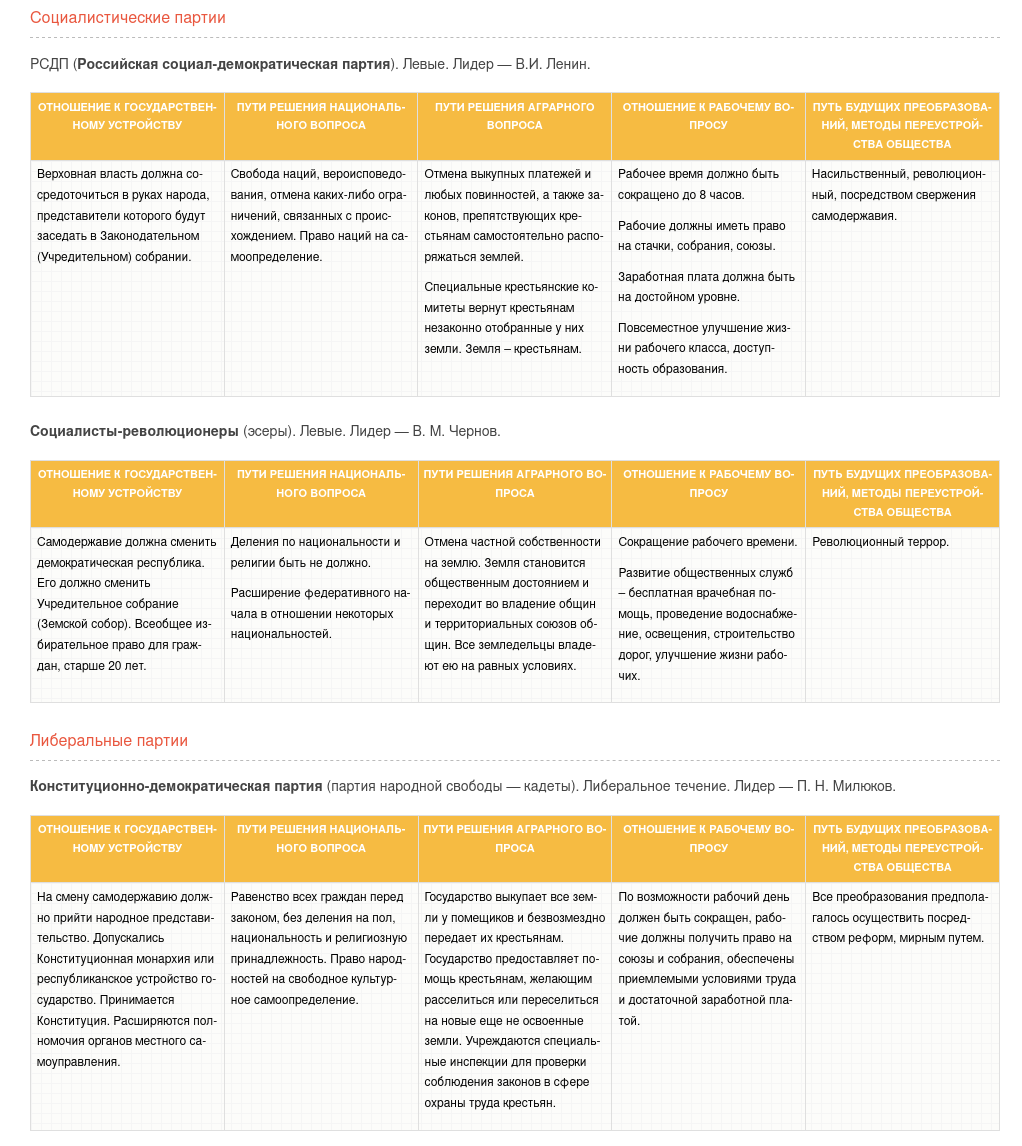
\includegraphics[width=\textwidth]{parties_01}

\pagebreak

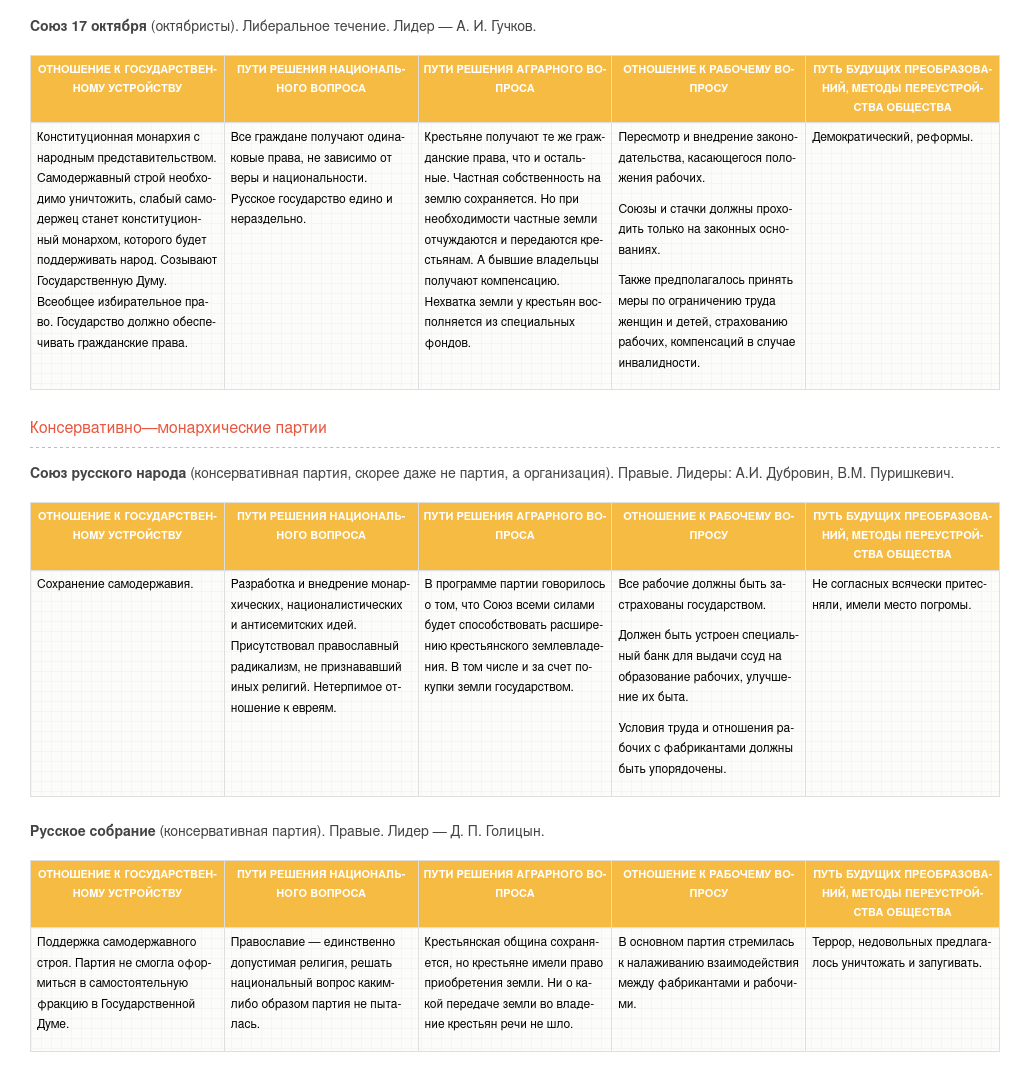
\includegraphics[width=\textwidth]{parties_02}

\pagebreak
\subsection{Политические портреты партийных лидеров}

\subsubsection{Социалистические партии}

\paragraph{Российская социал-демократическая партия (РСДП), Владимир Ильич Ленин}

\paragraph{Социалисты-революционеры (эсеры), Виктор Михайлович Чернов}

\subsubsection{Либеральные партии}

\paragraph{Конституционно-демократическая партия (партия народной свободы — кадеты), Павел Николаевич Милюков}

\paragraph{Союз 17 октября (октябристы), Александр Иванович Гучков}

\subsubsection{Консервативно-монархические партии}

\paragraph{Союз русского народа, Александр Иванович Дубровин}

\paragraph{Русское собрание, Дмитрий Петрович Голицын}

\subsection{Причины Первой мировой войны и ее основные этапы}

Непосредственным поводом начала военных действий принято считать \textbf{Сараевское убийство эрцгерцога Франца Фердинанда сербским националистом Гаврилой Принципом}. С другой стороны, столь же общепризнано, что \textbf{убийство было лишь ближайшим поводом, «толчком» к войне}, в то время как к ней исподволь вели многочисленные скрытые факторы, центральными из которых являлось \textbf{желание Германской империи господствовать в мире и конкурирующие национальные интересы крупнейших европейских держав}. 

\subsubsection{Основные этапы Первой мировой войны}

\paragraph{Первый (маневренный)}

В начале войны все стороны привели в движение свои огромные армии. Тут стоит вспомнить, что коммуникации в начале XX века были развиты не очень хорошо, так что маневрирование и передвижение отнимало много времени, счёт шёл на недели и месяцы. Первый этап Первой мировой войны продлился около года, \textbf{с лета 1914 года} (когда Австро-Венгрия объявила войну Сербии, а Россия в ответ начала всеобщую мобилизацию войск) \textbf{до лета 1915 года}. Масштабных сражений в это время не было, но боестолкновения и битвы относительно небольшого масштаба случались, когда противоборствующие стороны прощупывали силы противника.

\hfill

Но было и одно исключение – \textbf{Галицийское сражение, одно из самых крупных во всей Первой мировой}. Оно состоялось в самом начале войны, в августе и сентябре 1914 года. \textbf{Российская армия разгромила армию Австро-Венгрии}. Успехи России обеспокоили Германию, и уже к весне 1915 года она сосредоточила основное внимание на Восточном фронте. Однако, несмотря на победу над австрийцами, все сражения с германской армией на этом этапе закончились для российских войск поражением. Несмотря на это, русское наступление на Восточную Пруссию помогло Франции (союзнице России) выстоять в самый тяжёлый для неё момент. Германии была навязана война на два фронта, что сорвало планы немецкого командования завершить войну блицкригом, то есть одним молниеносным броском с серией военных операций.

\paragraph{Второй (позиционный)}

К началу второго этапа Первой мировой войны \textbf{сложились устойчивые фронты}. \textbf{Западный фронт} прошёл через Бельгию, Люксембург, а также территории Германии и северо-востока Франции. После провала попытки немцев стремительным натиском захватить Францию фронт стал позиционным, он протянулся от Северного моря до франко-швейцарской границы и остался неизменным почти до конца войны. \textbf{Восточный фронт} был менее позиционным, но гораздо более протяжённым, и на нём прошли многие крупнейшие сражения второго этапа Первой мировой войны.

\hfill

\textbf{Россия воевала именно на Восточном фронте}, но после революции она начала подготовку к выходу из войны, что и было проделано после подписания \textbf{Брестского мира в марте 1918 года}. Зимой 1916 года Германия запросила мира, но просьба эта была отклонена, так как условия мира не удовлетворяли английским, французским и даже русским амбициям. Война была продолжена, что означало скорый и полный разгром истощенной Германии и ее ослабленных союзников – Австро-Венгрии и Болгарии, и победу Антанты (Союза России, Франции и Англии), получавшей к этому времени значительную поддержку от США, на чем собственно и завершается позиционный период в войне, после которого Германия перешла к явному отступлению.

\paragraph{Третий (завершающий)}

Несмотря на то, что \textbf{Германия и её союзники явно сдавали позиции}, погрузившаяся в хаос из-за революции Россия не могла продолжать сражаться. Русские войска отступали с захваченных позиций, которые они удерживали долгое время. По результатам сепаратного Брестского мира Россия обязалась выплатить Германии репарации, но её это уже не могло спасти. \textbf{Германскую армию теснили на всех фронтах – Западный, Восточный, Африканский}. Колонии Германии в Тихом океане (острова Самоа) также были захвачены австралийскими и новозеландскими войсками. В 1918 году Германия предприняла так называемое \textbf{Весеннее наступление} и даже добилась определённых успехов, но закрепить и развить их не сумела. В целом третий период Первой мировой войны был для немецких войск неблагоприятным. 

\hfill

Преимущество Германии и её союзников в живой силе и технике окончательно сошло на нет после того, как США вступили в войну на стороне Антанты. Переломный момент наступил в \textbf{битве при Пьяве (17 – 23 июня 1918 года)}, когда войска Антанты нанесли сокрушительное поражение Австро-Венгрии и перешли к масштабному наступлению. Уже в Августе войска Антанты начали так называемое «стодневное наступление», которое представляло собой серию военных операций, в основном очень успешных. Именно это наступление привело к скорому поражению Германии и её союзников. Третий этап Первой мировой завершился \textbf{11 ноября 1918 года}, когда она официально закончилась.

\pagebreak
\subsection{Цели России в войне}

Официальная версия о причине начала Россией военных действий – это \textbf{выполнение союзнических обязательств перед Сербией}. Действительно, Россия, согласно договору, должна была оказать военную помощь Сербии в случае посягательств на территориальную целостность последней. 

\textbf{28 июля 1914 года Австро-Венгрия объявила войну Сербии}, и в тот же день начала обстрел Белграда. Россия события не торопила, отреагировав только спустя два дня – \textbf{31 июля, когда в стране была объявлена всеобщая мобилизация}. Германия в ультимативной форме потребовала от России отменить мобилизацию, но получила отказ.

1 августа немецкий посол в Петербурге граф Фридрих Пурталес передал \textbf{ноту об объявлении войны} российскому министру иностранных дел Сергею Сазонову, после чего, по воспоминаниям министра, «отошел к окну и заплакал». 2 августа уже Николай II подписал манифест о начале войны.

\hfill

Президент Российской ассоциации историков Первой мировой войны \textbf{Сергеев Евгений Юрьевич} (профессор, доктор исторических наук) отмечает, что решение России вступить в войну было продиктовано также ее \textbf{«боязнью потерять престиж и влияние в Балканских странах»}. Сербия была не просто союзником, но и важным стратегическим плацдармом на Балканах. 

Историк \textbf{Борис Иванович Колоницкий} (профессор, доктор исторических наук) убежден в том, что анализируя причины начала войны, не стоит недооценивать значение общественного мнения. \textbf{По его словам, имело место «сильное давление улицы»}. Окружение Николая II отмечало, что царь в те дни ощущал такое единение с народом, какого не было за все предыдущие 20 лет его правления.

\textbf{В первые дни войны на улицах российских городов прошли массовые манифестации в поддержку сербов}, не обошлось и без стихийных погромов немецких офисов и магазинов. Антигерманские настроения и патриотическая эйфория оказались фактором, во многом предопределившим вступление России в войну.

\hfill

Американский историк \textbf{Шон Макмикин} (кандидат наук) объясняет мотивы Первой мировой войны \textbf{соперничеством и территориальными претензиями России и Германии}. Эту мысль подкрепляет французский дипломат \textbf{Морис Палеолог} в книге «Царская Россия во время мировой войны», приводя слова российского министра иностранных дел Сергея Сазонова: «Моя формула проста, мы \textbf{должны уничтожить германский империализм}. Мы достигнем этого только рядом военных побед; перед нами длинная и очень тяжелая война. Император не имеет никаких иллюзий в этом отношении. Но чтобы «кайзерство» не восстановилось снова из своих развалин, чтобы Гогенцоллерны никогда больше не могли претендовать на всемирную монархию, должны произойти большие политические перемены».

\textbf{Борис Колоницкий} высказывает мнение, что целью России было \textbf{объединение польских территорий, входящих в состав Австро-Венгрии и Германии, а также необходимость установления контроля над Босфором}. Записка, адресованная Сазоновым французскому и британскому послам (М. Палеологу и Дж. Бьюкенену), подтверждает, что в преддверие ожидавшейся атаки союзных войск на Босфор Россия поспешила \textbf{«застолбить»} за собой Константинополь и Проливы. В ней, в частности, сказано следующее: «Ход последних событий приводит императора Николая к мысли, что вопрос о Константинополе и проливах должен быть окончательно разрешен и сообразно вековым стремлениям России».

Об этом же в своей книге «Взгляд Запада на Россию» пишет британский историк \textbf{Джеффри Хоскинг} (почетный доктор Института Российской истории РАН): «К весне 1915 года русские дипломаты наконец-то достигли соглашения с правительствами Великобритании и Франции о том, что \textbf{после войны Константинополь и большая часть проливов станут территорией России}».

\pagebreak
\subsection{Социально-экономическая и политическая обстановка в России в годы Первой мировой войны}

\href{https://studme.org/1911052216224/istoriya/sotsialno-ekonomicheskaya_politicheskaya_obstanovka_rossii_gody_voyny}{Статья «Социально-экономическая и политическая обстановка в России в годы войны»}

\pagebreak
\subsection{Власть, общество и человек в годы войны}{Статья «Власть и общество России во время Первой мировой войны»}

\href{https://histerl.ru/kurs_sssp/podrobno/vlasti_obshestvo_v_godi_voini.htm}{Статья «Власть и Общество в годы войны»}

\end{document}